\include{settings}

\begin{document}	% начало документа

% Титульная страница
\begin{titlepage}	% начало титульной страницы

	\begin{center}		% выравнивание по центру

		\large Санкт-Петербургский политехнический университет Петра Великого\\
		\large Физико-механический институт \\
		\large Высшая школа прикладной математики и вычислительной физики\\[3cm]
		% название института, затем отступ 6см
		\large Направление подготовки\\
		\large "01.03.02. Прикладная математика и информатика"\\[3cm]
		\huge Дисциплина "Численные методы"\\[0.5cm] % название работы, затем отступ 0,5см
		\large Отчет по лабораторной работе №4\\[0.1cm]
		\large "Решение алгебраической проблемы собственных значений итерационными методами. Степенной метод для поиска второго максимального по модулю собственного значения и соответствующего собственного вектора"\\[5cm]

	\end{center}


	\begin{flushright} % выравнивание по правому краю
		\begin{minipage}{0.25\textwidth} % врезка в половину ширины текста
			\begin{flushleft} % выровнять её содержимое по левому краю

				\large\textbf{Работу выполнил:}\\
				\large Иванова А.С.\\
				\large {Группа:} 5030102/00002\\
				
				\large \textbf{Преподаватель:}\\
				\large Курц В.В.

			\end{flushleft}
		\end{minipage}
	\end{flushright}
	
	\vfill % заполнить всё доступное ниже пространство

	\begin{center}
	\large Санкт-Петербург\\
	\large \the\year % вывести дату
	\end{center} % закончить выравнивание по центру

\end{titlepage} % конец титульной страницы

\vfill % заполнить всё доступное ниже пространство


\include{ToC}

\section{Формулировка задачи}

Дана функция 
\begin{math} 
	y=\sqrt{\sin{x^{2}}}
\end{math}



Требуется вычислить определенный интеграл заданной функции на нескольких отрезках квадратурными формулами Гаусса с 3 узлами. Исследовать влияние заданной точности на объем вычислений, влияние гладкости функций на точность вычислений. Сравнить результаты с результатами для метода Симпсона.

\section{Алгоритм метода и условия его применимости}

\subsection{Алгоритм метода}

Дана функция, которую нужно интегрировать на отрезке [a;b] и количество интервалов, на которое разбивается отрезок N. 

Рассмотрим квадратурные формулы. Представим определенный интеграл на промежутке [a;b] функции F(x) в виде:


Пусть 

\begin{math} 
	\int\limits_{a}^{b}F(x)dx=\int\limits_{a}^{b}p(x)f(x)dx
\end{math}

Формулы вида:

\begin{math} 
	\\
	\int\limits_{a}^{b}p(x)f(x)dx=\sum\limits_{k=1}^{N}A_{k}f(x_{k})dx \\
	A_{k} , x_{k}
\end{math}
- коэффициенты и узлы квадратурной формулы. 



\begin{math} 
	\int\limits_{a}^{b}f(x)dx=\frac{h}{3}(f(x_{0})+4\sum\limits_{i=1}^{N}f(x_{2i-1})+2\sum\limits_{i=1}^{N-1}f(x_{2i})+f(x_{2N}))
\end{math}

За счет выбора узлов и коэффициентов можно ожидать алгебраический порядок точности 2n-1. Узлы можно менять по формуле Родрига, где они являются корнями полинома Лежандра.

\begin{math} 
	[a;b]=[-1;1] => P_{n}(x)=c_{n}\frac{d^{n}}{dx^{n}}[(1-x^{2})^{n}] 
\end{math}

В случае для трех узлов: 

\begin{math} 
	\\
    P_{3}(x)=c_{3}\frac{d^{3}}{dx^{3}}[(1-x^{2})^{3}] = c_{3}\frac{d^{3}}{dx^{3}}[1-3*x^{2}-3*x^{4}-x^{6}]= c_{3}[3*4*3*2*x-6*5*4*x^{3}]=0 \\
    3x-5x^{3}=0 => x(3-5x^{2})=0 => x_{1}=-\sqrt{0.6}; x_{2}=0; x_{3}=\sqrt{0.6}
\end{math}

Кэффициенты можно найти через систему определяющих уравнений: 

\begin{equation}
	\begin{cases}
		A_{1}+A_{2}+A_{3}= \int\limits_{-1}^{1} x^{0}dx=2 \\
		A_{1}x_{1}+A_{2}x_{2}+A_{3}x_{3}=\int\limits_{-1}^{1} x^{1}dx=0 \\
		A_{1}x_{1}^{2}+A_{2}x_{2}^{2}+A_{3}x_{3}^{2}=\int\limits_{-1}^{1} x^{2}dx=\frac{2}{3} \\
	\end{cases}
\end{equation}

Коэффициенты: 

\begin{math} 
	\\ 
	A_{1}=A_{3}=\frac{5}{9}; A_{2}=\frac{8}{9}
\end{math}

Получаем: 

\begin{math} 
	\\ 
	\int\limits_{-1}^{1}F(x)dx \approx \frac{1}{9}[5F(-\sqrt{0.6})+8F(0)+5F(\sqrt{0.6})]
\end{math}

Для того, чтобы найти интеграл на произвольном отрезке [a;b]

\begin{math} 
	\\ 
	t = \frac{a+b}{2}+\frac{b-a}{2}*x \\
	\int\limits_{a}^{b}F(t)dt = \frac{b-a}{2} \int\limits_{-1}^{1}F(\frac{a+b}{2}+\frac{b-a}{2}*x)dx \approx \frac{b-a}{2} \sum\limits_{k=1}^{N}A_{k}f(\frac{a+b}{2}+\frac{b-a}{2}*x_{k}) \\
	\int\limits_{a}^{b} F(x)dx \approx \frac{b-a}{18} (5F(\frac{a+b}{2}-\frac{b-a}{2}*\sqrt{0.6})+8F(\frac{a+b}{2}) +5F(\frac{a+b}{2}+\frac{b-a}{2}*\sqrt{0.6}))
\end{math}

Обобщенная формула для отрезка с разбиениями 

\begin{math} 
	h=\frac{b-a}{N}; t_{k}=a+h*k, k=0,...,N \\
	\int\limits_{a}^{b} F(x)dx \approx \sum\limits_{i=1}^{N} \frac{h}{18} \sum\limits_{k=1}^{N} = A_{k}*F(5F(\frac{t_{i-1}+t_{i}}{2}-\frac{t_{i}-t_{i-1}}{2}*\sqrt{0.6})+8F(\frac{t_{i-1}+t_{i}}{2}) +5F(\frac{t_{i-1}+t_{i}}{2}+\frac{t_{i}-t_{i-1}}{2}*\sqrt{0.6}))
\end{math}

Для оценки погрешности используется правило Рунге:

\begin{math} 
	\frac{|S_{n,2N}(f)-S_{n,N}(f)|}{2^{m}-1} \leq \epsilon
\end{math}

Для формулы Гаусса m=2*n-1=2*3-1=5

\subsection{Условия применимости метода}

Функция должна быть непрерывна на заданном участке.

\section{Предварительный анализ задачи}

Заданная фукнция не является непрерывной на всей области определения. Следовательно необходимо выбирать те участки, где функция будет непрерывна. Также данная функция имеет разрывы производных всех порядков. 

\section{Проверка условий применимости метода}

Заданная фукнция не является непрерывной на всей области определения. Следовательно необходимо выбирать те участки, где функция будет непрерывна. 

\section{Тестовый пример с детальными расчетами для задачи малой размерности}

Возьмем функцию \begin{math} 
	f(x)=6x^{5}+5x^{4}+4x^{3}+3x^{2}+2x+1
\end{math}

Интервал: \begin{math} 
	[0;1]
\end{math}

Значение интеграла: 

\begin{math} 
	\int\limits_{0}^{1}(6x^{5}+5x^{4}+4x^{3}+3x^{2}+2x+1)dx=6
\end{math}

Найдем значение по формуле Гаусса для 3-х узлов. Поскольку алегбраический порядок точности метода равен 5, значение должно точно совпадать с реальным значением интеграла.
 
\begin{math} 
	S_{3}(f)=(5f(\frac{1}{2}-\frac{1}{2}*\sqrt{0.6})+8f(\frac{1}{2}) +5f(\frac{1}{2}+\frac{1}{2}*\sqrt{0.6}))= \frac{108.000}{18}=6.000
\end{math}

Значение совпадает с аналитически вычесленным значением интеграла.  
  
\section{Перечень контрольных тестов для иллюстрации метода}

Дана функция 
\begin{math} 
	y=\sqrt{\sin{x^{2}}}
\end{math}
Данная функция имеет в основном периодическую область определения, разрывов производной на области определения нет, производная не существует на тех участках, где не существует действительных значений исходной функции. 

Существует единственный разрыв производной в области опеределения - это точка [0,0]

Выбирались два отрезка [-0.01;0.5] и [0.5;1.01], входящие в область определения функции. Первый имеет разрыв производной при х=0. Для этих отрезков вычисляется определенный интеграл методом Гаусса для 3-х узлов. Исследуется количество необходимых итераций для достижения заданной точности и зависимость ошибки вычисления (вычиляется по правилу Рунге) от количества проделанных итераций (сходимость метода) для данных отрезков. 

\section{Модульная структура программы}

def my\_func(x):

\includegraphics[scale=0.75]{block1.pdf}

def Gauss3 (func, a, b):

\includegraphics[scale=0.75]{block2.pdf}


def number\_of\_iterations(eps ,func ,a , b,method):

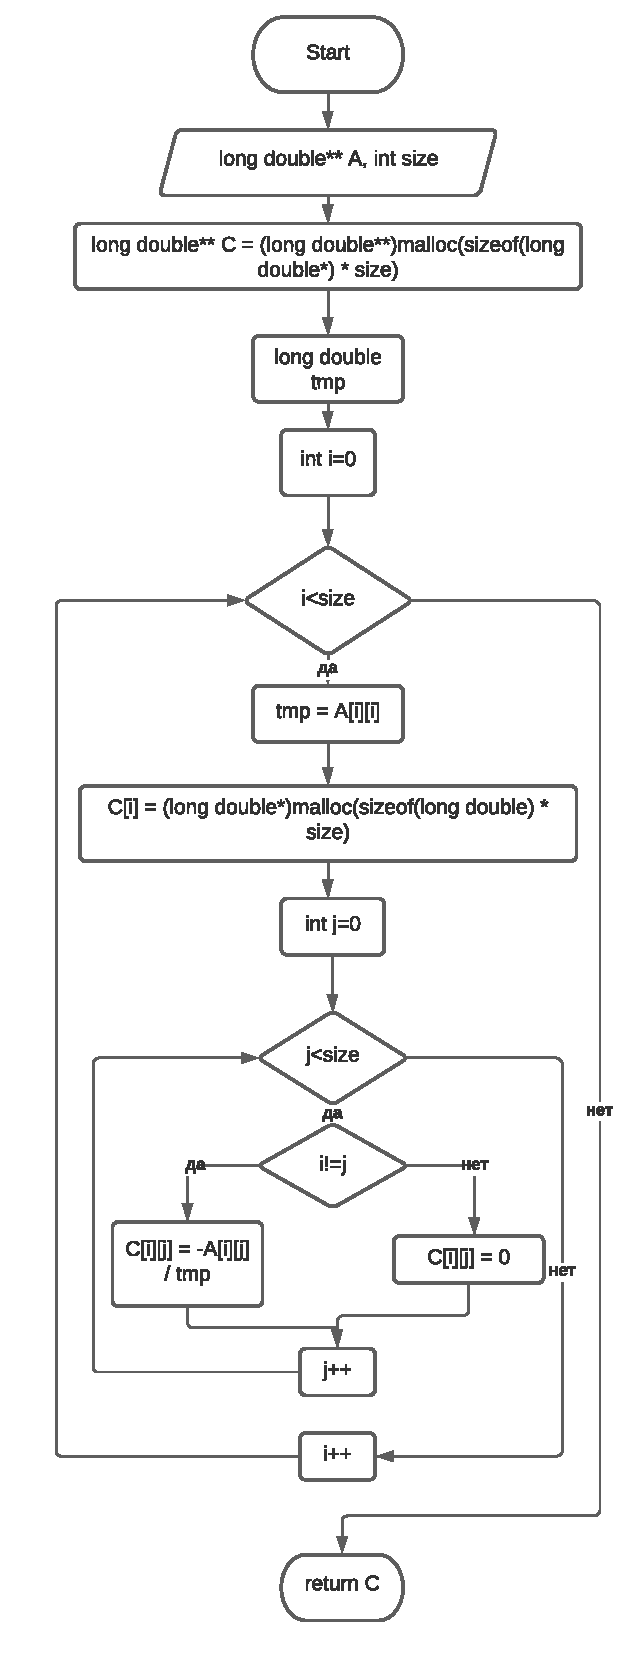
\includegraphics[scale=0.9]{block3.pdf}

def epsilon(numberiter ,func ,a , b, method):

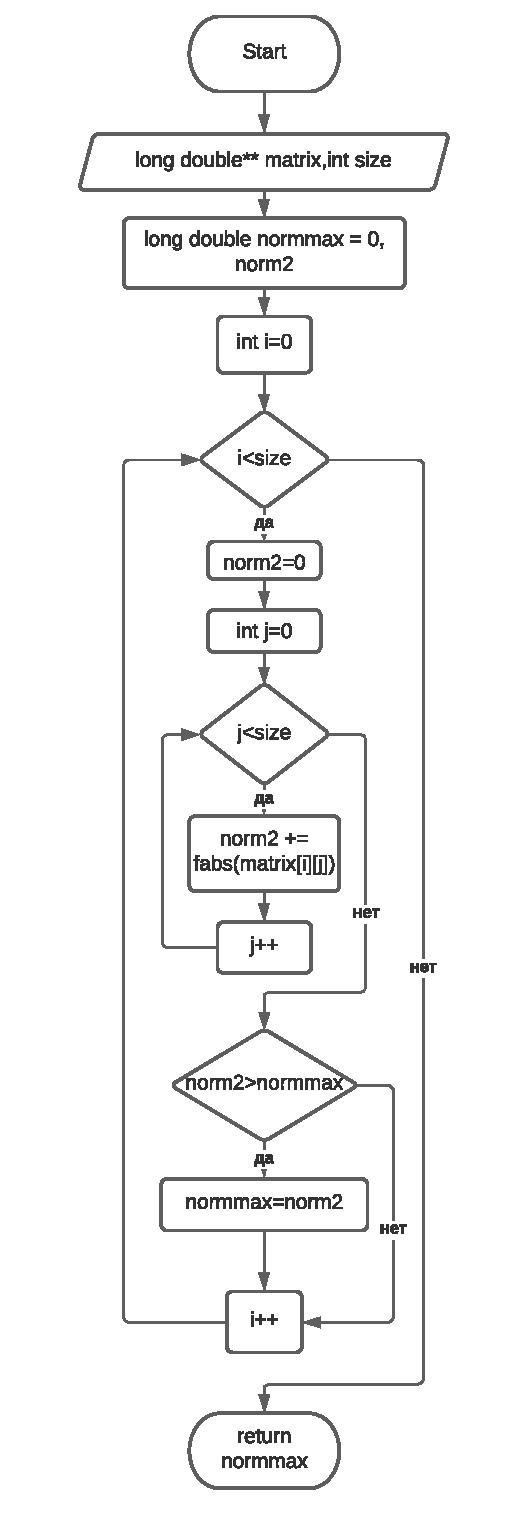
\includegraphics[scale=0.85]{block4.pdf}



\section{Численный анализ решения задачи}


\subsection{Зависимость количества итераций от заданной точности}

\includegraphics[scale=0.75]{1.pdf}

Как видно из данного графика, метод Гаусса для 3-х узлов требует меньшего количества итераций для достижения заданной точности, чем метод Симпсона, что обусловлено более выскоим алгебраическим порядком точности. Для обоих методов результаты для гладкого учатска функции лучше, чем для участка с разрывом производной. 

\subsection{Сходимость метода}

\includegraphics[scale=0.75]{2.pdf}

Как видно из данного графика, при увеличении количества итераций ошибка вычислений уменьшается, но до определнного момента. Начиная с некоторого количества итераций, ошибка вычислений начинает возрастать. Это обусловлено тем, что при больших n накапливается вычислительная ошибка.

Для графика сходимости метода Гаусса для трех узлов на участке с разрывом производной наблюдаются скачки результатов, что может быть обусловлено значениями функции на данном промежутке. 

\section{Краткие выводы}

На основе полученных результатов можно сделать вывод, что квадратурные формулы Гаусса хоть и требуют больших вычислительных затрат на каждой итерации, чем метод Симпсона, достигают заданной точности за меньшее количество итераций, чем формула Симпсона. Это обусловлено тем, что у метода Гаусса выше алгебраический порядок точности (5 для трех узлов, в то время, как у метода Симпсона - 3). при больших N накапливается вычислительная ошибка для обоих методов, что приводит к тому, что ошибка результата начинает увеличиваться. Следовательно с помощью обобщенных формул Симпсона и Гаусса можно достичь лишь некоторой точности (примерно 10е-16 для формул Симпсона и 10е-17 для формул Гаусса для 3 узлов для заданной функции),после чего увеличение количества итераций ухудшает результат. Для гладких участков функции необходимой точности можно достичь за меньшее количество итераций, чем для участков с разрывом производной для обоих методов.

\end{document}
